% Robótica 2026/2027 — Entrega 1, grupo Baldaia–Lavos, PL2.
% Compilar duas vezes para atualizar o índice e as referências.
\documentclass[10pt,a4paper]{article}
\usepackage[utf8]{inputenc}
\usepackage[T1]{fontenc}
\usepackage[portuguese]{babel}
\usepackage{lmodern}
\usepackage{geometry}
\geometry{left=17mm,right=17mm,top=17mm,bottom=18mm}
\usepackage{amsmath,amssymb,booktabs,array,graphicx,caption,hyperref,tikz}
\usetikzlibrary{arrows.meta}
\hypersetup{colorlinks=true,urlcolor=blue,linkcolor=blue}
\setlength{\parindent}{0pt}
\setlength{\parskip}{3pt}
\captionsetup{font=small,skip=3pt}
\newcommand{\source}[1]{\texttt{#1}}
\newcommand{\repo}{https://github.com/Baldaia12/RoboticaBaldaiaLavos/blob/windows/robotica-BaldaiaLavos}
\begin{document}
\begin{center}
{\Large\bfseries Robótica — Entrega 1: LW0, LW1 e LW2}\\[2mm]
Bernardo Pereira (2022219048) e João Lavos (2021222529), PL2\\
Ano letivo 2026/2027 \quad UFACTORY Lite 6
\end{center}
\vspace{-3mm}
\tableofcontents
\vspace{1mm}
\clearpage
\section{LW0 Parte 1 — Operar o Lite 6}
\textbf{Evidência:} leituras do Studio e SDK registadas pelo grupo, scripts \source{logs\_joints.py} e \source{safe\_session.py}, dados \source{juntas\_30s.csv}. A sessão segura é entregue também como código.

\subsection{Ligação e Live Control}
Na sessão documentada foi usada a rede \source{Robot-1}; o controlador tinha IP \source{192.168.1.182}, o portátil \source{192.168.1.12/24}, e o Studio foi acedido no porto \source{18333}. O primeiro erro observado foi \emph{Controller Error Code C2 — The Emergency Stop button is pushed in to Stop}. Depois de libertar a paragem, limpar o erro e ativar o braço, foi possível operar em modo de posição.

\begin{center}\small
\begin{tabular}{@{}lcc@{}}\toprule
Junta & Especificação/controlador (graus) & Extremos observados (graus)\\\midrule
J1 & $[-360,360]$ & $[-360,360]$\\
J2 & $[-150,150]$ & $[-143{,}3,148{,}6]$\\
J3 & $[-3{,}5,300]$ & $[-2{,}7,299{,}9]$\\
J4 & $[-360,360]$ & $[-360,360]$\\
J5 & $[-124,124]$ & $[-121{,}7,122{,}1]$\\
J6 & $[-360,360]$ & $[-360,360]$\\\bottomrule
\end{tabular}
\captionof{table}{Gamas da ficha e extremos ensaiados; os extremos observados não redefinem os limites.}
\end{center}

No referencial Base executaram-se X+, Y+, Z+, RX+, RY+ e RZ+, nessa ordem. A tabela transcreve as leituras de posição (mm) e orientação (graus) após cada comando; as translações avançaram 1 mm no eixo solicitado, enquanto as rotações mantiveram a posição e alteraram a orientação apresentada.
\begin{center}\small
\begin{tabular}{@{}lrrrrrr@{}}\toprule
Comando & $x$ & $y$ & $z$ & Roll & Pitch & Yaw\\\midrule
Inicial & $-2{,}6$ & $-261{,}7$ & $257{,}0$ & $174{,}5$ & $-38{,}0$ & $-29{,}7$\\
X+ & $-1{,}6$ & $-261{,}7$ & $257{,}0$ & $174{,}5$ & $-38{,}0$ & $-29{,}7$\\
Y+ & $-1{,}6$ & $-260{,}7$ & $257{,}0$ & $174{,}5$ & $-38{,}0$ & $-29{,}7$\\
Z+ & $-1{,}6$ & $-260{,}7$ & $258{,}0$ & $174{,}5$ & $-38{,}0$ & $-29{,}7$\\
RX+ & $-1{,}6$ & $-260{,}7$ & $258{,}0$ & $175{,}6$ & $-37{,}5$ & $-30{,}4$\\
RY+ & $-1{,}6$ & $-260{,}7$ & $258{,}0$ & $175{,}0$ & $-36{,}7$ & $-30{,}0$\\
RZ+ & $-1{,}6$ & $-260{,}7$ & $258{,}0$ & $175{,}0$ & $-36{,}7$ & $-29{,}0$\\\bottomrule
\end{tabular}
\captionof{table}{Leituras do Studio na sequência de comandos cartesianos.}
\end{center}
As rotações também alteraram várias juntas; estas leituras, por si só, não determinam uma convenção de Euler. O Studio indicou estado \emph{Normal}, modo \emph{Position} e montagem \emph{Floor}, com carga TCP de $0{,}28$ kg e juntas $[250{,}7,-4{,}2,49{,}0,-313{,}0,50{,}8,251{,}8]^\circ$. Com a carga definida, o braço foi guiado à mão e manteve a posição ao ser largado. A garra abriu e fechou; não foram registadas medições com paquímetro.

Durante o ensaio surgiu \emph{C22 — Self-collision Error}. No contacto com a bancada, o controlador emitiu \emph{C31 — Abnormal current in the robotic arm}, junta 2, com binário teórico de $10{,}661$ N\,m e real de $-32{,}36$ N\,m; o movimento foi interrompido. A recuperação observada foi limpar o erro, ativar, repor modo e estado. A sensibilidade de colisão registada foi 3, com carga de $0{,}277$ kg e centro de massa $[0,0,30]$ mm.

\subsection{Cinco exercícios Python}
\begin{enumerate}\setlength{\itemsep}{1pt}
\item \textbf{Leitura antes/depois do ensino:} com \source{get\_servo\_angle()} e \source{get\_position()}, as juntas passaram de $[250{,}7,-4{,}2,49{,}0,-313{,}0,50{,}8,251{,}8]^\circ$ para $[291{,}0,-4{,}2,49{,}0,-261{,}7,91{,}4,339{,}0]^\circ$. A pose passou de $[-1{,}6,-260{,}6,258{,}1,174{,}9,-36{,}7,-29{,}0]$ para $[217{,}6,-160{,}3,394{,}3,-82{,}2,15{,}2,-70{,}7]$ (mm e graus).
\item \textbf{Gamas:} os limites lidos do controlador coincidiram com a especificação da tabela acima.
\item \textbf{Home:} de três configurações iniciais, \source{set\_servo\_angle(..., speed=20, wait=True)} regressou a $[291,-4{,}2,49,-261{,}7,91{,}4,339]^\circ$. As partidas foram $[341{,}915,6{,}498,49,-254{,}400,91{,}400,339]$, $[257{,}582,-4{,}200,32{,}737,-261{,}700,91{,}400,339]$ e $[297{,}525,3{,}650,49,-248{,}089,69{,}308,316{,}976]^\circ$. Nas leituras finais impressas, a dispersão entre chegadas foi $0^\circ$ e o maior desvio absoluto foi $0{,}000020^\circ$; isto caracteriza as leituras do controlador, não a repetibilidade física independente.
\item \textbf{Cartesianas:} \source{set\_position()} aumentou Z de $394{,}182739$ para $444{,}182678$ mm ($\Delta z=49{,}999939$ mm) e regressou a $394{,}182800$ mm.
\item \textbf{Garra:} \source{open\_lite6\_gripper()}, \source{close\_lite6\_gripper()} e \source{stop\_lite6\_gripper()} foram aceites; o programa terminou com código 0.
\end{enumerate}

\subsection{Exemplos do SDK e registo temporal}
O exemplo \source{0002-get\_property} leu estado 2, modo 0, erros e avisos 0, pose e ângulos; foi adaptado o IP, sem movimento. O \source{2001-move\_joint} foi adaptado ao Lite 6: em vez das poses do xArm6, J1 avançou de $291{,}129768^\circ$ para $293{,}129792^\circ$ e voltou, com $10^\circ$/s, pausas e verificações de retorno. Assim foram exercitados \source{get\_servo\_angle()} e \source{set\_servo\_angle()} sem reutilizar limites de outro braço.

\begin{center}
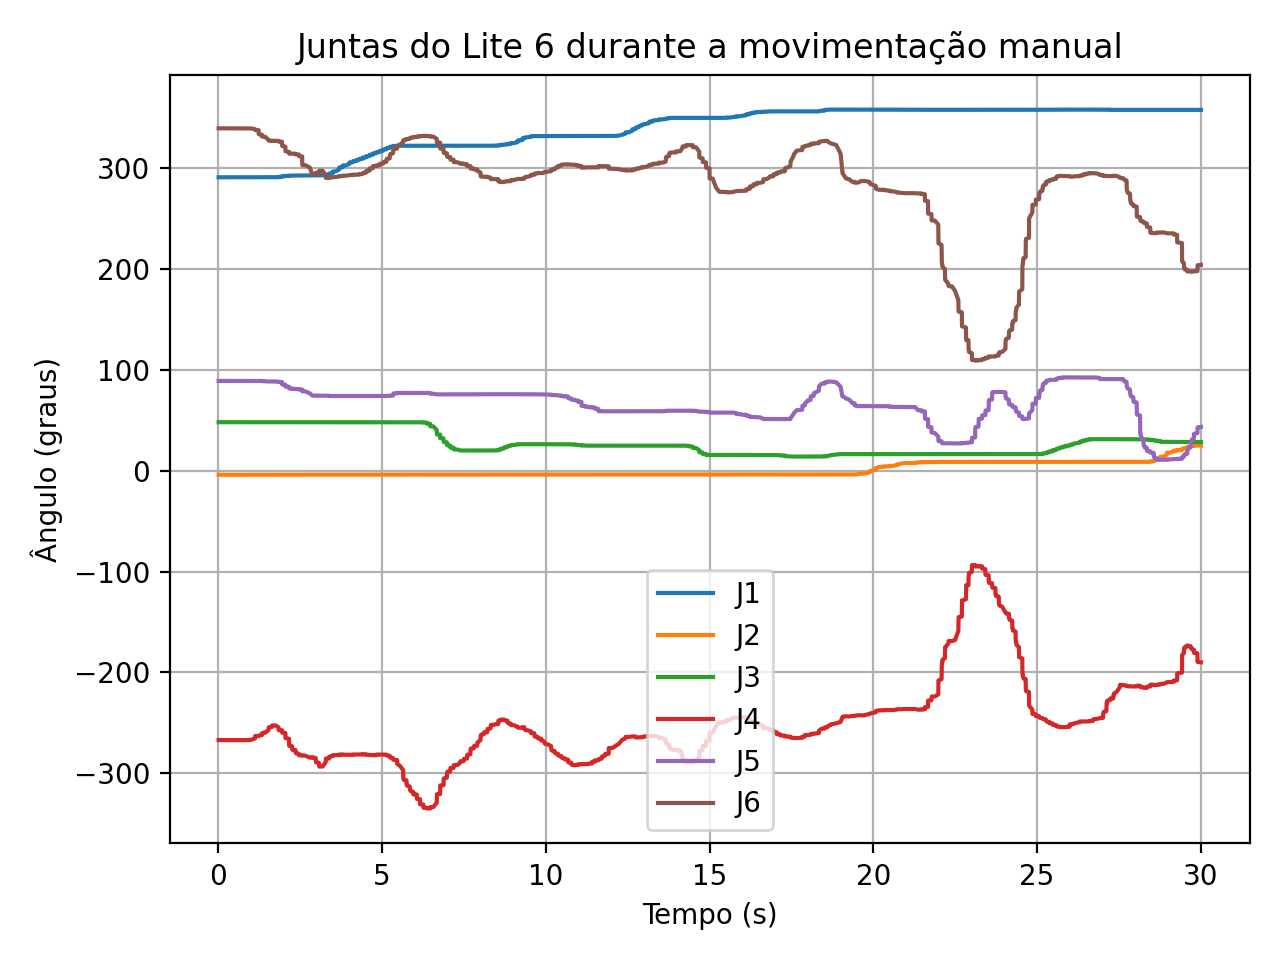
\includegraphics[width=0.78\linewidth,height=0.27\textheight,keepaspectratio]{images/lw0_juntas_30s.png}
\captionof{figure}{Ângulos das seis juntas durante orientação manual (gráfico original do grupo).}
\end{center}
O registo contém 1712 amostras em 30,00 s, sem pausa deliberada: $f_s=(N-1)/(t_{\mathrm{fim}}-t_{\mathrm{início}})=57{,}03$ amostras/s. As maiores variações visuais ocorrem em J4 e J6. A \source{safe\_session()} entregou a sessão com modo reduzido ativo, limites de $54^\circ$/s nas juntas e 150 mm/s no TCP e fronteira $[300,0,200,-200,400,10]$ mm.

\clearpage
\section{LW0 Parte 2 — Ambiente e ciclo de vida}
\textbf{Evidência:} logs e ficheiros em \source{lw0/parte2/}. Estes ensaios foram feitos em simulação; a validação física das LW1/LW2 é relatada nas secções próprias.

\subsection{Níveis escolhidos e validação do ambiente}
Foi usado o nível intermédio em Windows (Python 3.12.10, ambiente virtual, SDK xArm e pacote local \source{lite6}) e o nível avançado pela via Docker com ROS 2 Jazzy, MoveIt 2 e Gazebo Harmonic. O simulador de firmware UFACTORY correu o perfil Lite 6 \source{6 9}, firmware v2.4.0, em \source{127.0.0.1}. O grupo usou \source{ROS\_DOMAIN\_ID=0}, por não lhe ter sido atribuído um número, conforme a informação registada.

Na verificação B.5, \source{pytest -q} passou cinco testes; a sessão segura ligou ao simulador, e o movimento \emph{start $\to$ home} devolveu código 0 em $0{,}67$ s, com erro máximo impresso de $0{,}000^\circ$. A configuração vem de \source{config/robot.yaml}; não há IP \source{192.168} fixo no Python. O repositório tem commits e instruções de reprodução.

\begin{center}\small
\begin{tabular}{@{}cllp{8.5cm}@{}}\toprule
Teste & Tema & Resultado & Evidência registada\\\midrule
1 & ROS 2 & PASSA & Listener recebeu \emph{Hello World}.\\
2 & Pacotes UFACTORY & PASSA & Dez pacotes encontrados.\\
3 & Modelo/RViz & PASSA & Lite 6 e MotionPlanning; estado global OK.\\
4 & Árvore TF & PASSA & PDF da cadeia \source{world} $\to$ \source{link\_base} $\to$ \source{link\_eef}.\\
5 & \source{tf2\_echo} & PASSA & Duas matrizes $4\times4$ e respetivas juntas (abaixo).\\
6 & Gazebo & PASSA & Formas visíveis e relógio a avançar.\\
7 & MoveIt/Gazebo & PASSA & \emph{Plan \& Execute} deslocou o Lite 6 no Gazebo.\\
8 & SDK/TF & PASSA & Código 0; diferença de posição de $0{,}200$ mm na pose A.\\\bottomrule
\end{tabular}
\captionof{table}{Testes C.5. Não houve falhas finais e, por isso, não há primeira mensagem de erro a transcrever para estes ensaios.}
\end{center}

\subsection{Teste 5 — duas transformações e juntas}
As matrizes seguintes são as leituras \source{tf2\_echo} guardadas em \source{docs/evidencias/}, arredondadas a três casas decimais, em metros. Não representam uma medição com precisão superior a esse arredondamento.
\begin{align*}
\mathbf q_A&=[0,0,0,0,0,0]\ \mathrm{rad},&
{}^0T_{6,A}&=\begin{bmatrix}1&0&0&0.087\\0&-1&0&0\\0&0&-1&0.154\\0&0&0&1\end{bmatrix},\\[1mm]
\mathbf q_B&=[0.858983,1.378099,1.051537,0.000070,-0.326669,0.858897]\ \mathrm{rad},&
{}^0T_{6,B}&=\begin{bmatrix}1&0&0&0.134\\0&-1&0&0.156\\0&0&-1&-0.024\\0&0&0&1\end{bmatrix}.
\end{align*}
Na pose B, as juntas correspondem a $[49{,}216,78{,}959,60{,}249,0{,}004,-18{,}717,49{,}211]^\circ$. A diferença de unidades é relevante: ROS 2 usa metros/radianos; o SDK usa mm/graus por omissão.

\subsection{Testes 7 e 8, e reprodução}
No teste 7, o Gazebo mostrou a execução com dinâmica pelo controlador simulado; o RViz mostrou o plano e o modelo cinemático, sem a física do simulador. No teste 8, o SDK devolveu $[87{,}0,0{,}0,154{,}2,180,0,0]$ (mm e graus) para A; a posição TF era $[87,0,154]$ mm. Logo, $\|\Delta\mathbf p\|=0{,}200$ mm à precisão dos números reportados.

Seguindo o README a partir de uma shell limpa, foram repetidos os testes Python e B.5, bem como os testes 1, 3 e 8. O B.5 terminou com erro máximo impresso de $0{,}000^\circ$; o listener recebeu \emph{Hello World}, o RViz apresentou o modelo com estado global OK e a repetição do teste 8 manteve $0{,}200$ mm. Os ficheiros de evidência incluem os logs do ciclo de vida, as matrizes e a árvore de frames.

\subsection{Exercício de ciclo de vida: requisitos e testes}
\begin{center}\scriptsize
\begin{tabular}{@{}llp{11.5cm}@{}}\toprule
ID / teste & Tipo & Requisito verificável\\\midrule
R1 / T-F1 & Funcional & \source{safe\_session} liga e deixa modo 0, estado diferente de 4 e sem erros.\\
R2 / T-F2 & Funcional & Fecha a ligação mesmo após exceção no bloco da sessão.\\
R3 / T-F3 & Funcional & \source{home} termina com código 0 e erro máximo $\leq0{,}5^\circ$ nas seis juntas.\\
P1 / T-P1 & Desempenho & Abertura em 10 repetições: limiar $<5$ s, alvo $<2$ s.\\
P2 / T-P2 & Desempenho & Regresso a home em 5 repetições: limiar $<15$ s, alvo $<8$ s.\\
I1 / T-I1 & Interface & Parâmetros de \source{robot.yaml}, sem IP fixo no Python; unidades SDK documentadas.\\
S1 / T-S1 & Segurança & Exceção durante movimento deixa estado 4, deriva $<0{,}05^\circ$ em 1 s, alvo não atingido.\\
S2 / T-S2 & Segurança & Velocidade acima do máximo provoca \source{ValueError}, sem movimento.\\\bottomrule
\end{tabular}
\captionof{table}{Requisitos associados a teste antes da execução.}
\end{center}

\begin{center}\scriptsize
\begin{tabular}{@{}llp{10.2cm}@{}}\toprule
Teste & Resultado & Medição / observação\\\midrule
T-F1 & PASSA & \source{connected=True}, modo 0, estado 2, erro 0.\\
T-F2 & PASSA & \source{connected=False} após exceção induzida.\\
T-F3 & PASSA & Código 0; erro máximo impresso $0{,}000^\circ$.\\
T-P1 & PASSA & Pior $1{,}09$ s, média $1{,}08$ s, $n=10$.\\
T-P2 & PASSA & Pior $0{,}67$ s, média $0{,}67$ s; 5/5 chegadas válidas.\\
T-I1 & PASSA & Teste automático: um teste passou.\\
T-S1 & PASSA & Estado $4\to4$, progresso $0{,}8^\circ$, deriva $0{,}000^\circ$, distância ao alvo $9{,}1^\circ$.\\
T-S2 & PASSA & Comando recusado, deslocação $0{,}000^\circ$.\\\bottomrule
\end{tabular}
\captionof{table}{Resultados registados no simulador de firmware, em \source{logs/lifecycle\_sim\_20261026\_170724.csv}.}
\end{center}

\subsection{Rastreabilidade e modelo em V}
\begin{center}\scriptsize
\begin{tabular}{@{}llll@{}}\toprule
Requisito & Módulo/função & Teste & Resultado\\\midrule
R1 & \source{session.py::safe\_session} & T-F1 & PASSA\\
R2 & \source{safe\_session}/\source{finally} & T-F2 & PASSA\\
R3 & \source{session.py::go\_home} & T-F3 & PASSA\\
P1 & \source{safe\_session} & T-P1 & PASSA, $1{,}09$ s\\
P2 & \source{go\_home} & T-P2 & PASSA, $0{,}67$ s\\
I1 & \source{config.py::load\_config} & T-I1 & PASSA\\
S1 & \source{safe\_session}/\source{set\_state(4)} & T-S1 & PASSA\\
S2 & \source{session.py::\_check\_speed\_cap} & T-S2 & PASSA\\\bottomrule
\end{tabular}
\captionof{table}{Cada requisito liga-se a implementação, teste e resultado.}
\end{center}

\begin{center}
\begin{tikzpicture}[scale=0.78,every node/.style={font=\scriptsize},>=Stealth]
\draw[very thick,->] (0,3.2)--(3.7,0); \draw[very thick,->] (3.7,0)--(7.4,3.2);
\node[above] at (3.7,3.45) {Desafio Final: requisitos e validação do sistema};
\node[left] at (0.4,3.0) {LW4: trajetória}; \node[right] at (7.0,3.0) {testes de integração};
\node[left] at (1.25,2.25) {LW3: velocidade}; \node[right] at (6.15,2.25) {testes de LW3};
\node[left] at (2.1,1.5) {LW2: IK}; \node[right] at (5.3,1.5) {testes de LW2};
\node[left] at (2.95,0.75) {LW1: FK}; \node[right] at (4.45,0.75) {TF, SDK e testes LW1};
\node[below] at (3.7,-0.15) {LW0: ambiente, segurança e testes B.5};
\end{tikzpicture}
\captionof{figure}{Modelo em V da UC: cada módulo é confrontado com uma verificação correspondente.}
\end{center}
\textbf{Conclusão.} Foram validados o nível intermédio e a via Docker do nível avançado: B.5, os oito testes C.5, os oito testes de ciclo de vida e a repetição a partir de uma shell limpa passaram no simulador usado. Cada requisito da sessão segura e do regresso a home tem implementação, teste e resultado rastreáveis na tabela acima.

\clearpage
\section{LW1 — Cinemática direta}
\textbf{Fontes:} \source{lw1\_medicoes.csv}, \source{lw1\_fk\_sim.csv}, \source{lw1\_fk\_real.csv}, esboço fornecido pelo grupo e folha de parâmetros UFACTORY. A implementação avaliada está em \source{src/lite6\_kinematics/lite6\_kinematics/forward\_kinematics.py}.

\subsection{Parte A — Referenciais e medição}
O referencial de base é \source{link\_base} e o terminal é \source{link\_eef}. A figura é o esboço original na configuração de juntas zero; foi fornecido com 267$\times$452 píxeis, pelo que a tabela numérica a seguir fixa os parâmetros. A implementação usa a convenção \textbf{DH standard}, conforme indicado pelo docente; a tabela e a ordem das transformações abaixo seguem essa convenção, embora os nomes das funções do template mantenham \source{dh\_table} e \source{mdh\_transform}.

\begin{center}
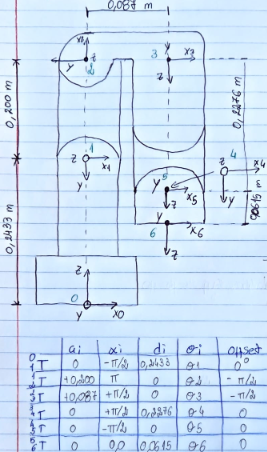
\includegraphics[height=0.31\textheight,keepaspectratio]{images/lw1_esboco.png}
\captionof{figure}{Esboço original das juntas, eixos, comprimentos e desvios angulares (LW1 A.1).}
\end{center}

A medição foi feita lendo apenas as juntas e a pose terminal em sete configurações: zero e uma rotação de cerca de $90^\circ$ por junta. O ficheiro guarda também quaternião, eixo $z$ terminal e código de erro (zero em todas as linhas). Não se usou URDF ou o modelo do Gazebo para extrair parâmetros.
\begin{center}\small
\begin{tabular}{@{}lrrrr@{}}\toprule
Configuração & $q$ variado & $x$ (mm) & $y$ (mm) & $z$ (mm)\\\midrule
zero & — & 87,00 & 0,00 & 153,59\\
J1 $+90^\circ$ & J1 & 0,00 & 87,00 & 153,59\\
J2 $+90^\circ$ & J2 & -89,91 & 0,00 & 156,50\\
J3 $+90^\circ$ & J3 & 290,12 & 0,00 & 530,69\\
J4 $+90^\circ$ & J4 & 86,99 & 0,00 & 153,59\\
J5 $+90^\circ$ & J5 & 24,50 & 0,00 & 216,09\\
J6 $+90^\circ$ & J6 & 87,00 & 0,00 & 153,59\\\bottomrule
\end{tabular}
\captionof{table}{Medições usadas na identificação geométrica.}
\end{center}
O ensaio de J1 confirma a rotação da projeção horizontal $(87,0)\to(0,87)$ mm. J4 e J6, na pose zero, mudam principalmente a orientação; J5 desloca a ponta de $(87,153{,}59)$ para $(24{,}5,216{,}09)$ mm no plano $xz$, dando escala de cerca de 62,5 mm para o avanço terminal. Os ensaios orientam a atribuição dos eixos e offsets; não identificam isoladamente todos os comprimentos com precisão submilimétrica. Para os valores nominais finais usou-se a tabela standard da folha do fabricante, comparada com estas observações.

\subsection{Tabela DH, comparação e implementação}
Na convenção standard, cada transformação é
\begin{equation}
{}^{i-1}T_i=R_z(q_i+\theta_{0,i})\,T_z(d_i)\,T_x(a_i)\,R_x(\alpha_i),
\qquad {}^0T_6=\prod_{i=1}^{6}{}^{i-1}T_i .
\end{equation}
\begin{center}\small
\begin{tabular}{@{}crrrr@{}}\toprule
$i$ & $a_i$ (m) & $\alpha_i$ & $d_i$ (m) & $\theta_{0,i}$\\\midrule
1 & 0 & $-\pi/2$ & 0,2433 & 0\\
2 & 0,2000 & $\pi$ & 0 & $-\pi/2$\\
3 & 0,0870 & $\pi/2$ & 0 & $-\pi/2$\\
4 & 0 & $\pi/2$ & 0,2276 & 0\\
5 & 0 & $-\pi/2$ & 0 & 0\\
6 & 0 & 0 & 0,0615 & 0\\\bottomrule
\end{tabular}
\captionof{table}{Tabela efetivamente implementada, com $\theta_i=q_i+\theta_{0,i}$ em radianos.}
\end{center}
Esta tabela coincide linha a linha com \emph{Standard D-H Parameters} da folha UFACTORY após converter mm para m e graus para radianos; a folha inclui também uma tabela \emph{Modified D-H Parameters}, com outra atribuição de referenciais e outra distribuição de $a$, $d$ e $\alpha$. Não se comparam linhas das duas convenções como se descrevessem o mesmo referencial intermédio. A pose terminal nominal em zero calculada por este modelo é $(87,0,154{,}20)$ mm; a medição e o TF do modelo são cerca de $(87,0,153{,}59)$ mm, diferença de cerca de $0{,}61$ mm em $z$. Esta discrepância entre parâmetros nominais e modelo de validação aparece nos erros medidos.

A função \source{dh\_table(q)} adiciona offsets ao vetor em radianos; \source{mdh\_transform()} constrói a matriz standard acima apesar do nome legado; \source{forward\_kinematics()} acumula as seis matrizes e, opcionalmente, devolve os sete referenciais. O nó \source{FkNode} lê juntas por nome de \source{/joint\_states} e publica a pose em \source{/lite6\_fk/pose}, copiando a marca temporal. Não se usou tf ou URDF no cálculo do grupo.

\subsection{Partes C e D — Verificação e validação}
Para uma pose calculada $(R_c,\mathbf p_c)$ e uma referência $(R_m,\mathbf p_m)$, foram usados os erros separados do enunciado:
\begin{equation}
e_p=\|\mathbf p_c-\mathbf p_m\|_2,\qquad
e_o=\arccos\!\left(\frac{\operatorname{tr}(R_c^\top R_m)-1}{2}\right).
\end{equation}
O \source{fk\_check} percorreu P0--P9 em Gazebo e depois no braço. A tabela mostra erros por configuração; os CSV incluem as juntas atingidas, matrizes e marcas temporais.
\begin{center}\scriptsize
\begin{tabular}{@{}lrrrrrr@{}}\toprule
& \multicolumn{2}{c}{Gazebo: vs. TF} & \multicolumn{2}{c}{Braço: vs. TF} & \multicolumn{2}{c}{Braço: vs. controlador}\\
Pose & mm & graus & mm & graus & mm & graus\\\midrule
P0 & 0,611 & 0,0008 & 0,611 & 0,0008 & 1,268 & 0,0078\\
P1 & 0,626 & 0,0012 & 0,626 & 0,0012 & 3,093 & 0,4697\\
P2 & 0,643 & 0,0013 & 0,643 & 0,0013 & 4,072 & 0,6291\\
P3 & 0,653 & 0,0011 & 0,653 & 0,0011 & 2,227 & 0,4154\\
P4 & 0,803 & 0,0014 & 0,803 & 0,0014 & 4,111 & 0,7393\\
P5 & 0,982 & 0,0010 & 0,982 & 0,0010 & 1,291 & 0,3851\\
P6 & 0,620 & 0,0009 & 0,620 & 0,0009 & 2,424 & 0,4135\\
P7 & 0,895 & 0,0014 & 0,895 & 0,0014 & 4,066 & 0,6837\\
P8 & 0,613 & 0,0010 & 0,613 & 0,0010 & 2,473 & 0,2132\\
P9 & 0,899 & 0,0010 & 0,897 & 0,0010 & 3,750 & 0,5318\\\midrule
Máximo & 0,982 & 0,0014 & 0,982 & 0,0014 & 4,111 & 0,7393\\\bottomrule
\end{tabular}
\captionof{table}{Erros por pose de \source{lw1\_fk\_sim.csv} e \source{lw1\_fk\_real.csv}; arredondamento apenas para apresentação.}
\end{center}
As dez posições foram registadas em cada ambiente, sem rejeição na execução real final. P1.3 (Gazebo vs. TF, $<2$ mm e $<0{,}05^\circ$) é cumprido, inclusive os alvos de $1{,}5$ mm e $0{,}01^\circ$. P1.4 exige comparação \emph{com o controlador real}, com limiar $<3$ mm e $<0{,}1^\circ$: o máximo medido de $4{,}111$ mm e $0{,}7393^\circ$ \textbf{não cumpre}. A concordância com TF não substitui essa referência. Os dados não permitem atribuir causa única à diferença; parâmetros/calibração do controlador, definição de TCP e instante de amostragem exigiriam investigação. P1.2 depende de referência e poses ocultas do docente; não é declarado aprovado com estes ficheiros.

\textbf{Vídeo.} \href{\repo/lw1/lw1_fk_real.mp4}{Execução da LW1 no braço}: o verificador pede confirmação antes de cada movimento e regista P0--P9. O ficheiro tem 90,24 s.

\clearpage
\section{LW2 — Cinemática inversa algébrica}
\textbf{Fontes:} CSV de \source{lw2/}, capturas E.2 e \source{src/lite6\_ik/lite6\_ik/inverse\_kinematics.py}. O modelo direto usado é o da LW1, na convenção DH standard, mantendo a pose de \source{link\_eef} em \source{link\_base}.

\subsection{Parte A.1 — Derivação da solução fechada}
Seja $T_d=[R_d\ \mathbf p_d;\,0\ 1]$. A ponta está a $d_6=0{,}0615$ m do centro do punho ao longo de $\hat z_6$; logo,
\begin{equation}
\mathbf p_w=\mathbf p_d-d_6R_d\mathbf e_z=(x_w,y_w,z_w)^\top,\quad
h=z_w-d_1,\quad \rho=\sqrt{x_w^2+y_w^2}.
\end{equation}
Com $L_1=a_2=0{,}200$ m, $L_2=\sqrt{a_3^2+d_4^2}=\sqrt{0{,}087^2+0{,}2276^2}$ m e $\beta=\operatorname{atan2}(a_3,-d_4)$, há dois ramos para a base:
\begin{equation}
(q_1,r)=\bigl(\operatorname{atan2}(y_w,x_w),\rho\bigr)
\quad\text{ou}\quad
\bigl(\operatorname{atan2}(y_w,x_w)+\pi,-\rho\bigr).
\end{equation}
No plano ombro--cotovelo--punho, a lei dos cossenos dá
\begin{equation}
c=\frac{r^2+h^2-L_1^2-L_2^2}{2L_1L_2},\quad
\delta=\pm\arccos\bigl(\operatorname{clip}(c,-1,1)\bigr),\quad
q_3=\beta-\delta,
\end{equation}
\begin{equation}
q_2=\operatorname{atan2}(r,h)-\operatorname{atan2}\!\left(L_2\sin\delta,L_1+L_2\cos\delta\right).
\end{equation}
Assim cada ramo de $q_1$ admite até dois ramos do cotovelo. A orientação das três primeiras juntas, deduzida do produto DH da LW1, é
\begin{equation}
R_{03}=\begin{bmatrix}
c_1c_v&s_1&-c_1s_v\\s_1c_v&-c_1&-s_1s_v\\-s_v&0&-c_v
\end{bmatrix},\quad
v=q_2-q_3,\quad R_{36}=R_{03}^{\top}R_d,
\end{equation}
com $c_i=\cos q_i$, $s_i=\sin q_i$, $c_v=\cos v$ e $s_v=\sin v$. Para o punho regular, $s=\sqrt{R_{36,13}^2+R_{36,23}^2}>0$ e cada sinal $\sigma\in\{+s,-s\}$ fornece
\begin{equation}
q_4=\operatorname{atan2}\!\left(-R_{36,23}/\sigma,-R_{36,13}/\sigma\right),\quad
q_5=\operatorname{atan2}(\sigma,R_{36,33}),\quad
q_6=\operatorname{atan2}\!\left(-R_{36,32}/\sigma,R_{36,31}/\sigma\right).
\end{equation}
Cada ângulo é reduzido a $(-\pi,\pi]$; vetores equivalentes módulo $2\pi$ dentro de $\varepsilon_s=10^{-6}$ rad são devolvidos uma só vez. O algoritmo não usa iteração nem otimização.

\subsection{Partes A.2–A.4 — Ramos, alcance e singularidades}
Num caso regular há até $2\times2\times2=8$ soluções: inversão da direção da base, dois cotovelos e duas configurações do punho (sinal de $q_5$). O alvo é geometricamente inalcançável quando $c<-1$ ou $c>1$; o código tolera $10^{-12}$ além desses limites para não perder uma solução na fronteira por arredondamento. Na fronteira os ramos do cotovelo podem coincidir e a deduplicação remove repetições.

Quando os eixos das juntas 4 e 6 se alinham ($|\sin q_5|<\varepsilon_w=10^{-6}$), a pose não determina $q_4$ e $q_6$ separadamente. Para $q_5=0$, só a soma $q_4+q_6$ fica fixa módulo $2\pi$; a convenção é $q_4=0$ e $q_6=\operatorname{atan2}(R_{36,21},R_{36,11})$. O ramo de eixos opostos ($q_5=\pi$) tem relação angular análoga, mas está fora da gama permitida da junta 5. Se a projeção do centro do punho no plano da base for nula, o azimute requer cuidado geométrico adicional; os ensaios guardados não constituem uma campanha específica dessa singularidade.

\subsection{Seleção e nó ROS 2}
Para cada solução matemática $\mathbf q$, \source{select\_solution} substitui cada $q_i$ pelo equivalente $q_i+2\pi k$ dentro de \source{JOINT\_LIMITS} mais próximo do valor atual $q_{a,i}$. Descarta a solução se alguma junta não tiver equivalente admissível; das restantes escolhe $\arg\min\|\mathbf q-\mathbf q_a\|_2$. Sem solução executável, devolve \source{None}. O nó lê \source{/joint\_states} e \source{/lite6\_ik/target}, publica em \source{/lite6\_ik/solution} com a marca temporal do alvo ou regista \source{unreachable}/\source{out\_of\_range} sem publicar.

\subsection{Partes C e D — Verificação em Gazebo e no braço}
\begin{center}\scriptsize
\begin{tabular}{@{}lclrrrrrr@{}}\toprule
& & & \multicolumn{2}{c}{Gazebo vs. TF} & \multicolumn{2}{c}{Braço vs. TF} & \multicolumn{2}{c}{Braço vs. controlador}\\
Pose & Sim. & Real & mm & graus & mm & graus & mm & graus\\\midrule
A & atingida & atingida & 1,105 & 0,00155 & 1,188 & 0,03965 & 2,933 & 0,55723\\
B & atingida & atingida & 0,616 & 0,00120 & 0,585 & 0,02905 & 3,292 & 0,46126\\
C & atingida & atingida & 0,631 & 0,00117 & 0,651 & 0,02969 & 2,551 & 0,48339\\
D & atingida & atingida & 0,618 & 0,00106 & 0,523 & 0,03986 & 3,788 & 0,56863\\
U & recusada & recusada & — & — & — & — & — & —\\\midrule
Máximo A--D & & & 1,105 & 0,00155 & 1,188 & 0,03986 & 3,788 & 0,56863\\\bottomrule
\end{tabular}
\captionof{table}{Resultado por pose. A posição é em mm; o erro angular é o ângulo da rotação relativa.}
\end{center}
Em ambos os ambientes houve quatro poses atingidas, uma recusada (U, fora do alcance), zero rejeitadas. U foi recusada sem executar movimento para essa pose: P2.6 = 2/2. P2.4 (Gazebo vs. TF, $<2$ mm / $<0{,}05^\circ$) cumpre, incluindo os alvos $1{,}5$ mm / $0{,}01^\circ$. P2.5 é contra o controlador real, $<3$ mm / $<0{,}1^\circ$: $3{,}788$ mm / $0{,}56863^\circ$ \textbf{não cumpre}. A concordância com TF no braço não altera esta conclusão. Os dados não isolam se a discrepância vem de calibração, definição de TCP ou amostragem temporal. P2.2 e P2.3 são testes ocultos do docente; os estudos internos não os substituem.

\subsection{E.1 — Número de soluções}
\source{ik\_study count} produziu 500 linhas: 500/500 com oito soluções e com o vetor de origem encontrado. O erro interno máximo foi $6{,}14\times10^{-13}$ mm de posição e $2{,}58\times10^{-13}$ graus de orientação, contra a FK do próprio grupo.
\begin{center}\small
\begin{tabular}{@{}crrrrrrrr@{}}\toprule
N.º dentro das gamas & 1 & 2 & 3 & 4 & 5 & 6 & 7 & 8\\\midrule
N.º de poses & 4 & 171 & 14 & 212 & 1 & 3 & 8 & 87\\\bottomrule
\end{tabular}
\captionof{table}{Histograma E.1; o histograma do número total é: oito soluções em 500 poses.}
\end{center}
O gerador usa configurações regulares dentro das gamas, por isso os ramos da base, do cotovelo e do punho aparecem sem colapso nas 500 poses. Uma reavaliação das 4000 soluções com os limites do template encontrou 1576 violações da junta 3, 416 da junta 5, 328 da junta 2, e 12, 37 e 40 das juntas 1, 4 e 6, respetivamente; uma solução pode violar mais de uma gama. A restrição assimétrica da junta 3 é a principal redução do número executável. A contagem reproduziu \source{n\_in\_range} nas 500 linhas.

\subsection{E.2 — Todas as configurações para a pose A}
\source{ik\_check -p all:=true} registou oito soluções, quatro dentro das gamas e executadas (1, 2, 5, 6). As restantes foram rejeitadas sem movimento. Ângulos em graus, arredondados a uma casa:
\begin{center}\scriptsize
\begin{tabular}{@{}cll@{}}\toprule
N.º & $[q_1,q_2,q_3,q_4,q_5,q_6]$ & Resultado\\\midrule
1 & $[-28{,}1,31{,}0,106{,}1,-96{,}0,77{,}9,18{,}9]$ & atingida\\
2 & $[-28{,}1,31{,}0,106{,}1,84{,}0,-77{,}9,-161{,}1]$ & atingida\\
3 & $[-28{,}1,89{,}6,-148{,}0,-85{,}0,77{,}4,-29{,}6]$ & fora das gamas\\
4 & $[-28{,}1,89{,}6,-148{,}0,95{,}0,-77{,}4,150{,}4]$ & fora das gamas\\
5 & $[151{,}9,-89{,}6,106{,}1,102{,}1,83{,}9,-71{,}5]$ & atingida\\
6 & $[151{,}9,-89{,}6,106{,}1,-77{,}9,-83{,}9,108{,}5]$ & atingida\\
7 & $[151{,}9,-31{,}0,-148{,}0,93{,}7,77{,}0,-24{,}0]$ & fora das gamas\\
8 & $[151{,}9,-31{,}0,-148{,}0,-86{,}3,-77{,}0,156{,}0]$ & fora das gamas\\\bottomrule
\end{tabular}
\captionof{table}{Soluções de A: pares 1/2 e 5/6 invertem o punho; 1/2 vs. 5/6 trocam o ramo da base. Os ramos 3/4 e 7/8 têm $q_3=-148^\circ$, abaixo do limite inferior da junta 3.}
\end{center}
\begin{center}
\begin{tabular}{@{}cc@{}}
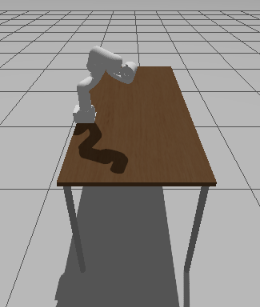
\includegraphics[width=0.39\linewidth,height=0.11\textheight,keepaspectratio]{images/E2_A_solucao_1.png} &
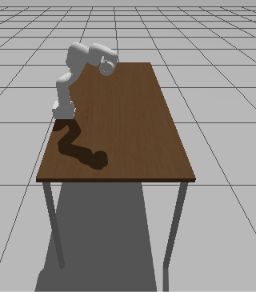
\includegraphics[width=0.39\linewidth,height=0.11\textheight,keepaspectratio]{images/E2_A_solucao_2.png}\\
Solução 1 & Solução 2\\
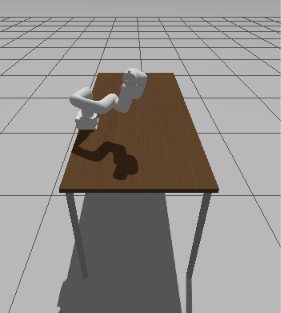
\includegraphics[width=0.39\linewidth,height=0.11\textheight,keepaspectratio]{images/E2_A_solucao_5.png} &
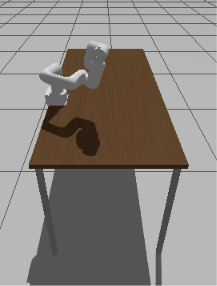
\includegraphics[width=0.39\linewidth,height=0.11\textheight,keepaspectratio]{images/E2_A_solucao_6.png}\\
Solução 5 & Solução 6
\end{tabular}
\captionof{figure}{Capturas do Gazebo fornecidas pelo grupo, uma por solução executada.}
\end{center}

\subsection{E.3 — Seleção a partir de S1–S4}
\begin{center}\small
\begin{tabular}{@{}clc@{}}\toprule
Arranque & Solução escolhida para A (graus) & Ramo E.2\\\midrule
S1 & $[-28{,}1,31{,}0,106{,}1,-96{,}0,77{,}9,18{,}9]$ & 1\\
S2 & $[-28{,}1,31{,}0,106{,}1,84{,}0,-77{,}9,-161{,}1]$ & 2\\
S3 & $[151{,}9,-89{,}6,106{,}1,102{,}1,83{,}9,-71{,}5]$ & 5\\
S4 & $[151{,}9,-89{,}6,106{,}1,-77{,}9,-83{,}9,108{,}5]$ & 6\\\bottomrule
\end{tabular}
\captionof{table}{Resultados dos quatro ficheiros \source{lw2\_ik\_sim\_A\_S1.csv} a \source{S4.csv}.}
\end{center}
Os quatro arranques colocam o braço perto de regiões diferentes do espaço articular. Depois do ajuste por $2\pi k$ e da exclusão dos ramos fora das gamas, a distância $\|\mathbf q-\mathbf q_{\mathrm{atual}}\|_2$ escolhe os ramos 1, 2, 5 e 6, respetivamente. A pose cartesiana final é a mesma; a proximidade articular muda.

\subsection{E.4 — Singularidade do punho}
\source{ik\_study wrist} registou 100 poses, sete soluções por pose (700 linhas). Em cada pose, uma das sete é a solução singular canónica com $q_4=0$ e $q_5=0$, conservando $q_4+q_6$ módulo $2\pi$. No primeiro caso, o vetor gerador tem $(q_4,q_6)=(-2{,}905177,0{,}944771)$ rad; a solução canónica devolve $(0,-1{,}960406)$ rad, a mesma soma. As outras seis soluções pertencem a outros ramos de base/cotovelo/punho e não precisam ter $q_5=0$. O erro interno máximo foi $9{,}92\times10^{-12}$ mm e $9{,}19\times10^{-12}$ graus, contra a FK do próprio grupo.

\textbf{Vídeo.} \href{\repo/lw2/lw2_ik_real.mp4}{Execução da LW2 no braço}: o verificador visita S0, executa A–D e regista U como recusada, sem comandar a pose fora do alcance. O ficheiro tem 66,32 s.

\end{document}
